\question The augmented cube $AQ_n$ is constructed as follows. First, $AQ_1$ consists of a link joining node 0 and node 1. Given $AQ_n$, where $n \geq 1$, we construct $AQ_{n+1}$ by taking two copies of $AQ_n$, call them $AQ_n^0$ and $AQ^1_n$, and renaming the nodes of $AQ_n^0$ (resp. $AQ_n^1$) by tagging $0$ (resp. 1) onto their names. A simple induction yields that for all $n \geq 1$, the node set of $AQ_n$ is $\{0,1\}^n$. Next, we join the node $(u_1, u_2, \ldots, u_n, 0)$ of $AQ_n^0$ with the node $(u_1, u_2, \ldots, u_n, 1)$ of $AQ_n^1$ and also the node $(\overline u_1, \overline u_2, \ldots, \overline u_n, 1)$ of $AQ^1_n$ where for any $b \in \{0,1\}$, $b = 0$ if and only if $\overline b = 1$. 
\begin{parts}
  \part What are the degrees of the nodes of $AQ_n$ for $n \geq 1$?
  [You should justify your claim.]
  \begin{solution}
    We look at $n = 1$, we have $AQ_1$ being isomorphic to $Q_1$, and thus $\deg(AQ_1) = 1$.
    Next, we assume $\deg(AQ_k) = 2k-1$ for some $k$. Now, we look at $AQ_{k+1}$. We can build this graph from two copies of $AQ_k$ by associating each node in one copy with two nodes in the other. Thus, we get $\deg(AQ_{k+1}) = \deg{AQ_k}+2 = 2(k+1)-1$. Thus, by induction, we have $\deg(AQ_n) = 2n-1$.
  \end{solution}

  \part Suppose that for some $n \geq 1$, any two nodes $x$ and $y$ of $AQ_n$ have $\min\{\deg_n(x), \deg_n(y)\}$ mutually node-disjoint paths joining them, where $\deg_n(x)$ (resp. $\deg_n(y)$) is the degree of $x$ (resp. $y$) in $AQ_n$. Suppose that $u = (u_1, u_2, \ldots, u_n, 0)$ and $v = (v_1, v_2, \ldots, v_n, 0)$ are two distinct nodes of $AQ_{n+1}$. Prove that $u$ and $v$ have $\min\{\deg_{n+1}(u), \deg_{n+1}(v)\}$ mutually node-disjoint paths joining them. 
  \begin{solution}
    Let $\bm u = (u_1, \ldots, u_n, 0)$ and $\bm v = (v_1, \ldots, v_n, 0)$ be nodes in $AQ_{n+1}$. Firstly, by viewing the first $n$ components of $\bm u$ and $\bm v$ in $AQ_n$, we can construct $2n-1$ node-disjoint paths (by assumption). So, to complete our proof we must find 2 more. Let
    \begin{align*}
      \bm v' &= (v_1, \ldots, v_n, 1), \\
      \bm v'' &= (\overline v_1, \ldots, \overline v_n, 1), \\
      \bm u' &= (u_1, \ldots, u_n, 1), \\
      \bm u'' &= (\overline u_1, \ldots, \overline u_n, 1).
    \end{align*}
    First, we assume that $n \geq 2$. Then we have two cases to look at.
    \begin{enumerate}
      \item Suppose that for all $i \in \{1, \ldots, n\}$, $u_i \neq v_i$. Then we must have $\bm u' = \bm v''$ (and $\bm u'' = \bm v'$). Thus we construct the addition (node-disjoint) routes:
      \begin{align*}
        &\bm u \to \bm u' = \bm v'' \to \bm v, \\
        & \bm u \to \bm u'' = \bm v' \to \bm v.
      \end{align*}

      \item Suppose otherwise. That is, there is $i \in \{1, \ldots, n\}$ such that $u_i = v_i$. We now consider the edges only in $Q_n$ (not that added edges from our construction), and partition this into two copies of $Q_{n-1}$ over dimension $i$. We see that $\bm u'$ and $\bm v'$ lie in the same partition, as do $\bm u''$ and $\bm v''$. Thus, as $Q_{n-1}$ is connected, we can construct two node-disjoint routes:
      \begin{align*}
        &\bm u \to \bm u' \to ... \to \bm v' \to \bm v, \\
        &\bm u \to \bm u'' \to ... \to \bm v'' \to \bm v
      \end{align*}
      as required.
    \end{enumerate}
    Finally, for the case when $n = 1$. We can trivially see that the condition holds.
  \end{solution}
\end{parts}

\question Prove that destination-tag routing in $2$-ary $n$-flies always yields a path from a given source to a given destination.
\begin{solution}
  Let $\bm s = (s_1, \ldots, s_n)$ be the source and $\bm d = (d_1, \ldots, d_n)$ be the destination. We first note that there are $n$ switch nodes. We see that when $\bm s$ reaches the switch node $i \in \{1, \ldots, n\}$, the edge that the route follows corresponds to the $i$th most significant bit of $\bm s$ (that is, $s_{n+1-i}$) being flipped or not flipped in order to match the $i$th most significant bit of $\bm d$. Thus, we can see that after moving through all $n$ switch nodes, each bit of our source \emph{must} equal our destination. So we have ensured our route ends at $\bm d$, but how can we be sure that the route is valid? By definition, the $i$th switch route has an edge in which no bits are flipped, or the $i$th most significant bit is flipped. Thus the route is well-defined. 
\end{solution}

\question \emph{Data centre networks} (DCNs) are interconnection networks for data centres and consist of interconnected servers and switches. Describe the difference between server-centric DCNs and switch-centric DCNs; in particular, explain any interconnection restrictions that occur and how routing is handled in both types of DCN. State one relative advantage of each type of DCN in comparison with the other. Say what a dual-port DCN is and explain why dual-port DCNs are important. Explain the \emph{stellar construction} of dual-port DCNs and how we can obtain routing algorithms in DCNs built using the stellar construction. Give an illustration of the stellar construction with a hypercube $Q_3$.
\begin{solution}
  A server-centric data centre network is such that the servers handle the routing; that is, algorithm-based. We are restricted by the processing speed on our router for calculating the routes for each packet. Alternatively, in a switch-centric data centre network, the switches handle the routing; that is, table-based. Here, we are restricted by the table size (memory). Switch-centric routing is fast in comparison to server-centric while server-centric routing is much more scalable.

  A dual-port data centre network is a data centre network in which each server has at most two ports. Dual-port data centres are important as most commercially available servers (as well as servers in existing data centres) have two ports (a primary and a backup). Thus, we can use reduce the building cost of our data centre by using cheaper and more basic equipment. 

  The \emph{stellar construction} of dual-port data centre networks is a method of constructing a dual-port data centre network (or \emph{stellar data centre network}) from any interconnection network. Let $G = (V, E)$ be an interconnected network where $V$ is the set of nodes are $E \in \mathcal P(V^2)$ is a set of links. The stellar data centre network $G^*$ is obtained by placing a switch-node $v^*$ for each $v \in V$, then placing 2 server-nodes $u^v, v^u$ for each $(u, v) \in E$ and adding a link between them (in $G^*$), then finally connecting $u^*$ to $u^v$ and $v^*$ to $v^u$.

  We now show how routes are transformed between a graph and its stellar construction. Given a route $P = (p_1, \ldots, p_n)$, we observe the route
  \[
    P^* = (p_1', p_1^*, p_1^{p_2}, p_2^{p_1}, p_2^*, \ldots, p_{n-1}^*, p_{n-1}^n, p_n^{n-1}, p_n^*, p_n')
  \]
  between $p_1'$ and $p_n'$, neighbours of the switch nodes $p_1^*$ and $p_2^*$ respectively. This path has size $2n+1$, but note, if $p_1' = p_1^{p_2}$ or $p_n^{n-1} = p'_n$, we can reduce our path size by 1 (and by 2 if both hold). Thus, if we have an efficient routing algorithm in our base graph, our stellar construction may inherit it.

  See below an illustration of the stellar construction with a hypercube $Q_3$.
  \begin{center}
    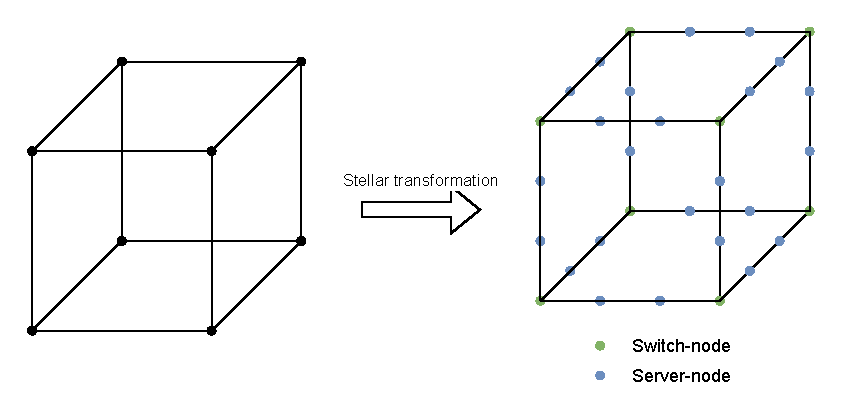
\includegraphics[width=0.8\textwidth]{q14.pdf}
  \end{center}
\end{solution}